

% \section{Dataset}
For our experiments, we use the \textit{impresso image classification} 
%impresso\_raw 
dataset\footnote{More specifically, we used collection under the \textit{impresso\_raw} folder from \url{https://github.com/impresso/impresso-image-classification}.} which originally consisted of 7,915 images classified into ten different classes, as presented in Figure \ref{tab:images_text}. 



% \begin{table}[h]
%     \centering
%     \begin{tabular}{cc|cc}
%         \hline
%         
\includegraphics[width=2cm]{report_title.png} & \raisebox{5\height}{title} & \includegraphics[width=2cm]{report_map.png} & \raisebox{4\height}{map} \\
%         
\includegraphics[width=2cm]{report_logo.png} & \raisebox{4\height}{logo} & \includegraphics[width=2cm]{report_game.png} & \raisebox{3\height}{game} \\
%         \includegraphics[width=2cm]{report_photo.png} & \raisebox{3\height}{photo} & \includegraphics[width=2cm]{report_graph.png} & \raisebox{2\height}{graph} \\
%         \includegraphics[width=2cm]{report_drawing.png} & \raisebox{.5\height}{drawing} & \includegraphics[width=2cm]{report_comic.png} & \raisebox{1\height}{comic} \\
%         \includegraphics[width=2cm]{report_diverse.jpg} & \raisebox{3\height}{diverse} & \includegraphics[width=2cm]{report_other.jpg} & \raisebox{3\height}{other} \\
%         \hline
%     \end{tabular}
%     \caption{Examples of images belonging to each class}
%     \label{tab:images_text}
% \end{table}

\begin{table}[h]
    \centering
    \begin{tabular}{ccccc}
        \hline
        
\includegraphics[width=2cm]{Images/class examples/report_title.png} & \includegraphics[width=2cm]{Images/class examples/report_map.png} & 
\includegraphics[width=2cm]{Images/class examples/report_logo.png} & \includegraphics[width=2cm]{Images/class examples/report_game.png} & \includegraphics[width=2cm]{Images/class examples/report_photo.png} \\
        title & map & logo & game & photo \\
        \includegraphics[width=2cm]{Images/class examples/report_graph.png} & \includegraphics[width=2cm]{Images/class examples/report_drawing.png} & \includegraphics[width=2cm]{Images/class examples/report_comic.png} & \includegraphics[width=2cm]{Images/class examples/report_diverse.jpg} & \includegraphics[width=2cm]{Images/class examples/report_other.jpg} \\
        graph & drawing & comic & diverse & other \\
        \hline
    \end{tabular}
    \caption{Examples of images belonging to each class.}
    \label{tab:images_text}
\end{table}

This dataset %was developed by Pauline Isabela Conti and 
contains a train set and a test set. The test set was mainly used, except for few-shot classification, where the examples given to the model were extracted from the train set. The statistics of this set are presented in Table \ref{tab:test-set}.

\begin{table}[h]
    \centering
    \begin{tabular}{lcccccccccc}
        \toprule
        \textbf{Class} & Title & Map & Logo & Game & Photo & Graph & Drawing & Comic & Diverse & Other \\
        \textbf{Count} & 81 & 17 & 46 & 46 & 375 & 37 & 90 & 41 & 64 & 5 \\
        \bottomrule
    \end{tabular}
    \caption{Class names with corresponding counts in the test set.}
    \label{tab:test-set}
\end{table}

After a few experiments, noticing that the classes “Diverse” and “Other” were too broad and overlapping with the other classes, we decided that it was not feasible to evaluate a classification task on them. The performance of the models achieved on those classes was not at all representative of the model's capabilities. They have thus been eliminated from the dataset used in this project.

